%%
%% This is file `sample-acmtog.tex',
%% generated with the docstrip utility.
%%
%% The original source files were:
%%
%% samples.dtx  (with options: `acmtog')
%% 
%% IMPORTANT NOTICE:
%% 
%% For the copyright see the source file.
%% 
%% Any modified versions of this file must be renamed
%% with new filenames distinct from sample-acmtog.tex.
%% 
%% For distribution of the original source see the terms
%% for copying and modification in the file samples.dtx.
%% 
%% This generated file may be distributed as long as the
%% original source files, as listed above, are part of the
%% same distribution. (The sources need not necessarily be
%% in the same archive or directory.)
%%
%%
%% Commands for TeXCount
%TC:macro \cite [option:text,text]
%TC:macro \citep [option:text,text]
%TC:macro \citet [option:text,text]
%TC:envir table 0 1
%TC:envir table* 0 1
%TC:envir tabular [ignore] word
%TC:envir displaymath 0 word
%TC:envir math 0 word
%TC:envir comment 0 0
%%
%%
%% The first command in your LaTeX source must be the \documentclass command.
\documentclass[acmtog]{acmart}

%%
%% \BibTeX command to typeset BibTeX logo in the docs
\AtBeginDocument{%
  \providecommand\BibTeX{{%
    \normalfont B\kern-0.5em{\scshape i\kern-0.25em b}\kern-0.8em\TeX}}}

%% Rights management information.  This information is sent to you
%% when you complete the rights form.  These commands have SAMPLE
%% values in them; it is your responsibility as an author to replace
%% the commands and values with those provided to you when you
%% complete the rights form.
\setcopyright{acmcopyright}
\copyrightyear{2018}
\acmYear{2018}
\acmDOI{10.1145/1122445.1122456}


%%
%% These commands are for a JOURNAL article.
\acmJournal{TOG}
\acmVolume{37}
\acmNumber{4}
\acmArticle{111}
\acmMonth{8}

%%
%% Submission ID.
%% Use this when submitting an article to a sponsored event. You'll
%% receive a unique submission ID from the organizers
%% of the event, and this ID should be used as the parameter to this command.
%%\acmSubmissionID{123-A56-BU3}

%%
%% The majority of ACM publications use numbered citations and
%% references.  The command \citestyle{authoryear} switches to the
%% "author year" style.
%%
%% If you are preparing content for an event
%% sponsored by ACM SIGGRAPH, you must use the "author year" style of
%% citations and references.
\citestyle{acmauthoryear}

%%
%% end of the preamble, start of the body of the document source.
\begin{document}

%%
%% The "title" command has an optional parameter,
%% allowing the author to define a "short title" to be used in page headers.
\title{A Tiny World: Atom}

%%
%% The "author" command and its associated commands are used to define
%% the authors and their affiliations.
%% Of note is the shared affiliation of the first two authors, and the
%% "authornote" and "authornotemark" commands
%% used to denote shared contribution to the research.
\author{Chung An, Chen}
\author{Yang, Liu}
\author{Linxi, Tao}

%%
%% By default, the full list of authors will be used in the page
%% headers. Often, this list is too long, and will overlap
%% other information printed in the page headers. This command allows
%% the author to define a more concise list
%% of authors' names for this purpose.
\renewcommand{\shortauthors}{Trovato and Tobin, et al.}

%%
%% The abstract is a short summary of the work to be presented in the
%% article.


%%
%% The code below is generated by the tool at http://dl.acm.org/ccs.cfm.
%% Please copy and paste the code instead of the example below.
%%

%%
%% This command processes the author and affiliation and title
%% information and builds the first part of the formatted document.
\maketitle

\section{Introduction}
Prior to the electron cloud model, there are a lot of attempts on building a theoretical model for an atom. Most of them, for example, the commonly known Rutherford-Bohr model, perceive the electrons as if they are planets orbiting the sun --- a non-changing centripetal movement. The electron cloud, however, models an atom consisting of a small, yet massive when put aside to its electrons, nucleus surrounded by a non-deterministic cloud of electrons.

In the electron cloud model, electrons can theoretically be found anywhere in the space. However, they can be found more often in some regions, which we usually call them orbitals despite no orbital motions of electrons are being held, than others. A Carbon atom has two orbitals, where the inner layer contains two electrons and the outer layer contains four, and electrons are less likely to be found in between the two layers.

This project aims to simulate and render a Carbon atom's presence in a three-dimensional space. The simulation will be grounded in the more accurate electron cloud model, shown in Figure 1 below. An electron cloud model depicts the occurence of an atom's electrons by a density map containing numerous sparse dots. In any region, the density of the dots draws a directly proportional relationship to the probability of an electron being present. To illustrate this model, We leverage a recently-built parallel programming language, namely \textbf{Taichi}, as our main development framework.

\begin{figure}[h]
  \centering
  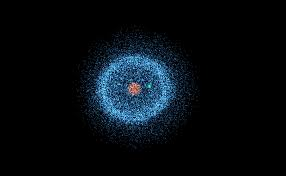
\includegraphics[width=\linewidth]{./concept_1.jpeg}
  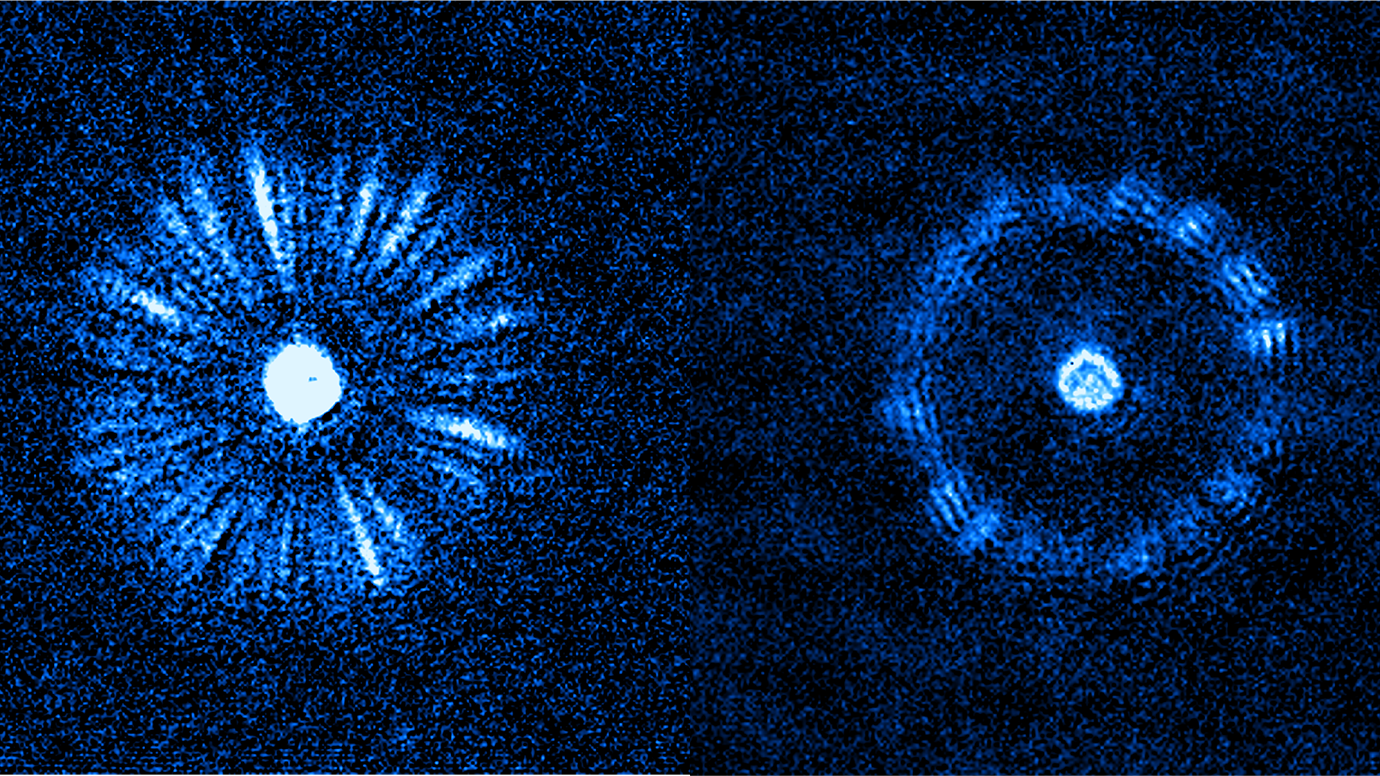
\includegraphics[width=\linewidth]{./concept_2.png}
  \caption{Atoms and Their Nucleus and Electron Cloud}
\end{figure}

\section{Software}
\textbf{Taichi} is a high-performance Domain-Specific Language for computer graphics applications. \textbf{Taichi} is designed towards performance, portability, spatially sparse computation, and differentiable programming. Despite inheriting most of its syntax from Python, \textbf{Taichi} does not carry over the downsides, for example, the slow computation speed, from Python.

\textbf{Taichi} is a higher level language such that it can be made to run on multiple mainstream rendering backends such as OpenGL, CUDA, and Metal. Using Pythonic decorators such as @ti.kernel and @ti.func brings the succeeding block of code into \textbf{Taichi}'s scope, where functions are naturally parallelized and differentiable on CPU or GPU devices. Two main data types in \textbf{Taichi} are Primitive Types and Compound Types. Primitive Types are numerical data types used by backends, while Compound Types are user-defined types composed of multiple members. To communicate between \textbf{Taichi}'s scope and Python's Scope, we use a global variables object called Field. They are commonly multi-dimensional array of elements of the following: a scalar, a vector, a matrix or a st, and can be either dense or sparse. Similar to a NumPy ndarray object, a field has a data type and a shape.





\end{document}
\endinput
%%
%% End of file `sample-acmtog.tex'.
